\documentclass[12pt,letterpaper]{article}
\usepackage{amsmath}
\usepackage{amsfonts}
\usepackage{amssymb}
\usepackage{enumitem}
\usepackage[left=2cm,right=2cm,top=3cm,bottom=3cm]{geometry}
\usepackage{natbib}
\usepackage{graphicx}
\usepackage{textcomp}
\usepackage{xcolor}
\usepackage[colorlinks = true,
            linkcolor = blue,
            urlcolor  = blue,
            citecolor = blue,
            anchorcolor = blue]{hyperref}

\newcommand{\MYhref}[3][blue]{\href{#2}{\color{#1}{#3}}}%
\newcommand{\textapprox}{\raisebox{0.5ex}{\texttildelow}}

\def\wl{\par \vspace{\baselineskip}}

\author{Abel Flores Prieto}
\title{Capstone Project Write Up - Cosmic Microwave Background Simulated Data}

\begin{document}
\maketitle

\section*{Scope}
This project focuses on the data used for computing the Cosmic Microwave
Background or CMB (see Figure \ref{fig:cmb}). In this project I focus to easily
enable access to data used for computing the CMB. The data used for this
project is simulated by \MYhref{https://arxiv.org/abs/0908.0540}{Sehgal et al.
(2010)} and can be found
\MYhref{https://lambda.gsfc.nasa.gov/simulation/tb\_sim\_ov.cfm\#2009}{here}.
This simulated data works as a tool to cross-check multiple calculations from
real surveys, including power spectrum calculations.

\begin{figure}[h!]
    \centering
    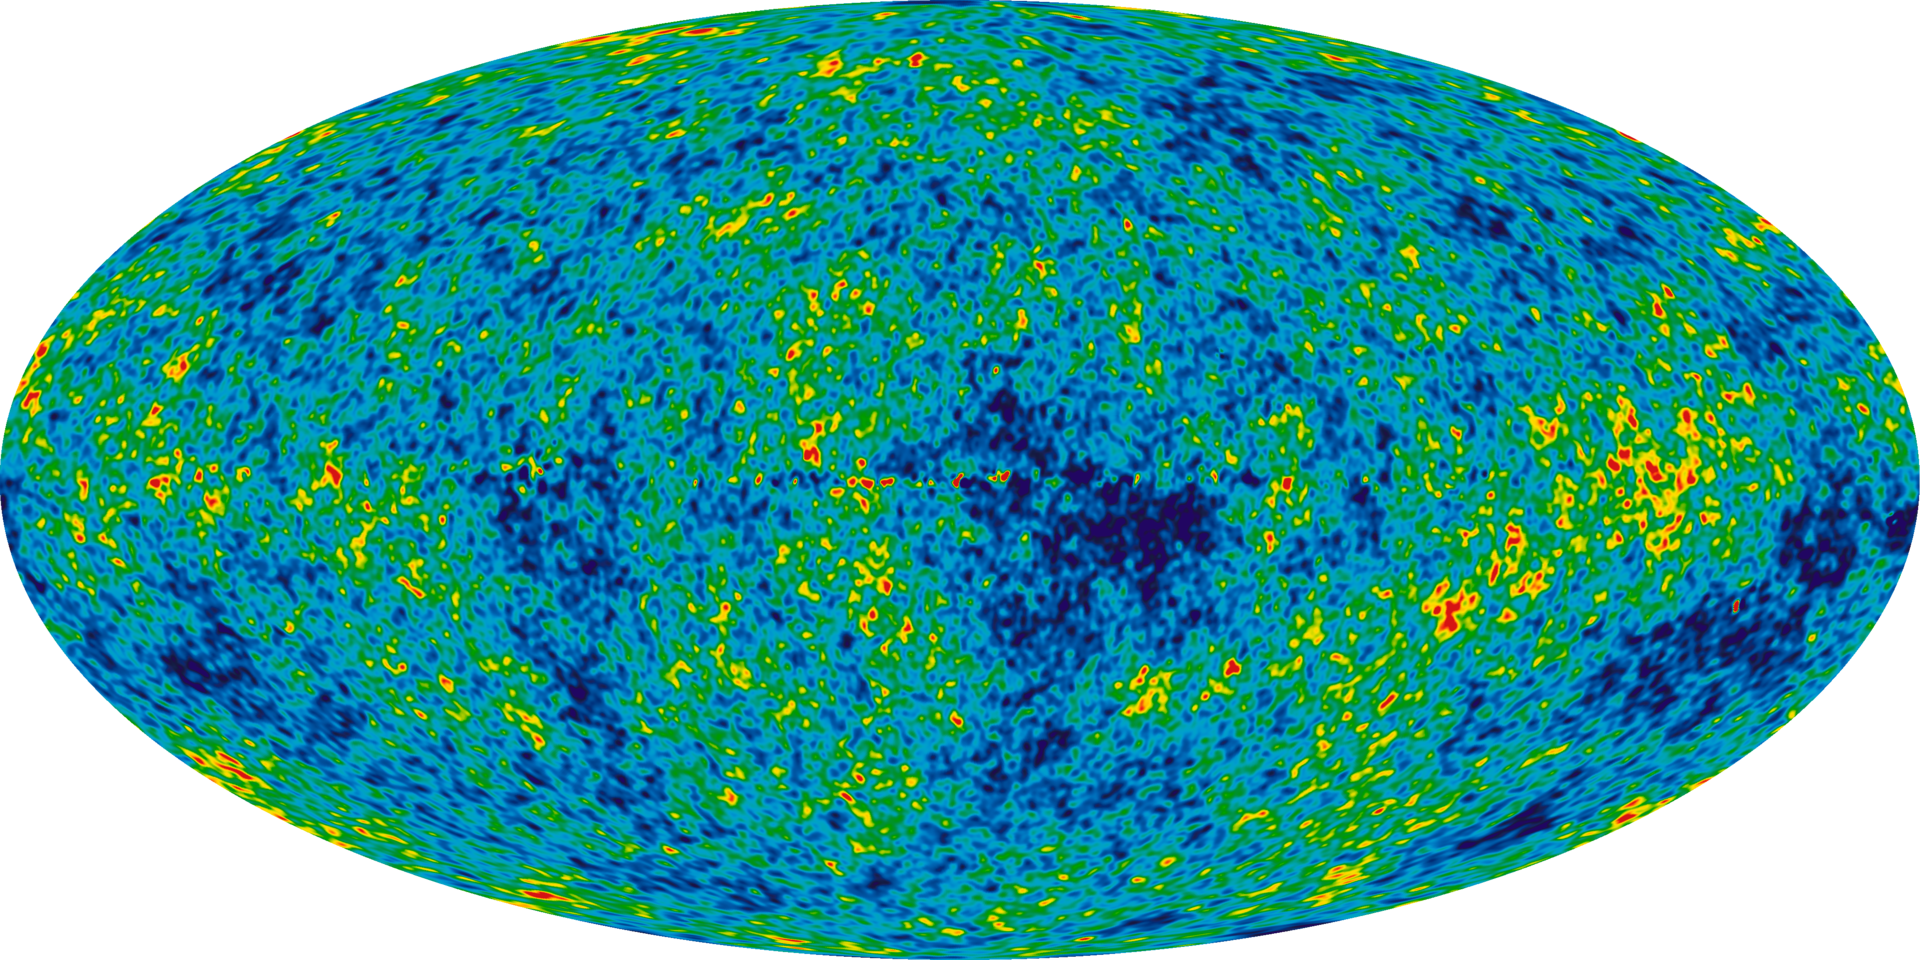
\includegraphics[width=0.75\textwidth]{imgs/cmb_temp.png}
    \caption{Cosmic Microwave Background temperature, remnant of the beginning
    of the universe. Image generated by NASA.}
    \label{fig:cmb}
\end{figure}

The data can be downloaded from the
\MYhref{https://lambda.gsfc.nasa.gov}{Legacy Archive for Microwave Background
Data Analysis}. The data used in this project is simulated by a team of
researchers and includes realistic simulations of the microwave sky. The data
is composed of Halo Catalogs and Galaxy Catalogs.

The galaxy catalogs come in DAT files with over 80 GB of data while the halo
catalogs come in as ASCII.GZ files with over 800 MB of data. All of this data
was uploaded to \texttt{s3://abelfp-physics-data-raw/}. The catalogs come with
a description of the data and what each column represents. These files can be
found under the \texttt{data/} directory in this project, all descriptions are
in TXT files.

This project will ensure that accessing
the data is easy by (1) transforming the data to parquet, (2) partitioning the
galaxy catalogs by frequency and data source, (3) and providing an easy way to
access the Halo catalogs for possibly joining to look at specific sources.

\subsection*{Galaxy Catalogs}
The Galaxy catalogs are divided in three sources: the Infrared High Flux
catalog with only \textapprox 300 galaxies, the Infrared Basic catalog with
\textapprox 600 M galaxies, and the Radio catalog with \textapprox 7 M
galaxies. Infrared High Flux and Infrared Basic share the same structure in the
data files. Both contain 10 columns with the following columns as specified in
their description file: \texttt{halo\_id}, \texttt{ra}, \texttt{dec},
\texttt{redshift}, and \texttt{f\_frequency} for the flux at the following
frequencies 30, 90, 148, 219, 277, 350 GHz in mJy units.  Infrared High Flux is
a single file at 39.3 KB, while Infrared Basic is composed of 11 files weighing
80 GB all together.  The data is numerical for all columns and is
space-seperated (not tab-seperated):

\begin{verbatim}
   29478    21.6392994    12.3277397     ...     527.6292114   967.6172485
   32523     0.6366578    43.5726509     ...     418.9460144   930.3469849
   33107    84.7412491    21.3145599     ...     338.1926880   649.5232544
   ...
\end{verbatim}

Similarly, the Radio catalog is also space-seperated, but it is missing the
column \texttt{halo\_id} and instead has an additional flux at 1.4 GHz. This is
a single file weighing 840.6 MB.

\subsection*{Halo Catalogs}
The Halo catalogs are also divided into three sources: Low Mass catalogs, High
Mass catalogs (NBody), and SZ Halo Catalog. Low and High Mass catalogs were in
the file format of ASCII.GZ files. These take a similar structure to the galaxy
catalogs, but with 20 columns as opposed to only 10. Togeher they weight over
500 MB.

\textbf{Note}: I did not include the SZ Halo catalog into the pipelines because
it required a lot more effort since it had 40 columns, and needed major
engineering effort.

\section*{Data Model}
For the data model I focused on the type of analysis that can be done on the
data. I would like to personally analyze the data, but the format of the files
from the website makes it hard to join all three galaxy sources, as well as
process in python or other software. It is also more time consuming to
analyze fluxes at different frequencies, since the frequency is specified in
the column name \texttt{f\_frequency}, as opposed to having its own column, and
a single column for \texttt{flux}.

\begin{table}[h!]
    \centering
    \begin{tabular}{ |c|c|c|c|c|c|c| }
        \hline
        halo\_id & ra & dec & redshift & f\_30 & f\_90 & f\_... \\
        \hline
        1 & 23.9 & 25.9  & 1.34 & 2.6 & 5.4 & 7.6 \\ 
        ... & ... & ...  & ... & ... & ... & ... \\ 
        \hline
    \end{tabular}
    \caption{Data model from original files for Galaxy catalogs.}
    \label{table:galold}
\end{table}

In the data model, I focused on transforming the flux columns into a single
column with an additional column reserved for frequency. See table
\ref{table:galold} for the model from original files, and table
\ref{table:galnew} for the new model.

\begin{table}[h!]
    \centering
    \begin{tabular}{ |c|c|c|c|c|c|c| }
        \hline
        halo\_id & ra & dec & redshift & frequency & flux & source\_type \\
        \hline
        1 & 23.9 & 25.9  & 1.34 & 30 & 5.4 & infrared\_basic\_simulated \\ 
        ... & ... & ...  & ... & ... & ... & ... \\ 
        \hline
    \end{tabular}
    \caption{Data model for transforming the data and saving as parquet.}
    \label{table:galnew}
\end{table}

For the \textbf{logical data model}, I structured the data in a data lake into
two tables: \texttt{cmb\_simulated} and \texttt{halo\_simulated}. The data is
stored in the S3 bucket \texttt{s3://abelfp-physics-data/} like so:

\begin{verbatim}
s3://abelfp-physics-data/
|-- data_lake/
    |-- cmb_simulated/
    |   |-- frequency=1.4/
    |   |   |-- source_type=radio_simulated/
    |   |       |-- part-00000-....snappy.parquet
    |   |       |-- part-00000-....snappy.parquet
    |   |-- frequency=30/
    |   |   |-- source_type=radio_simulated/
    |   |   |    |-- part-00000-....snappy.parquet
    |   |   |    |-- part-00000-....snappy.parquet
    |   |   |--- source_type=infrared_basic_simulated/
    |   |   |    |-- part-00000-....snappy.parquet
    |   |   |    |-- part-00000-....snappy.parquet
    |
    |-- halo_simulated/
        |-- part-00000-....snappy.parquet
        |-- part-00000-....snappy.parquet
\end{verbatim}

The end solution of the project is to have a data lake in S3 so that I, or
anyone (with the right permissions) can access the data for further processing.
The way the data is provided in the website makes it very hard to load and
process because of how massive some files are. It would also take a lot of
effort to combine the data. If I want to focus on a specific frequency for the
flux, that also involves extra work. Though the frequency is a not a string,
usually with these types of simulations, frequencies are finite, so it makes
sense to put it as a partition.

The halo catalog is not partitioned, but it is provided in parquet format
joining low and high mass halos.

The model for the halo catalog remained the same. See the configuration file
\texttt{configuration/configurations\_galaxies.py} to see the list of fields.
You can find it under the variable \texttt{halo\_low\_high\_columns}.

\section*{Run Pipelines to Model the Data}
For the project I chose to use Spark (PySpark), AWS EMR, and S3. I chose to use
Spark because the volume of the data is large with more than half a billion
rows. It seemed like the right tool to use for handling such massive amount of
data. With AWS EMR, it is easy to submit jobs and see if the cluster terminated
with errors or completed the job successfully. You can see the files
\texttt{bin/create\_submit\_emr\_job.sh} for how I submit the job with the AWS
CLI. Also take a look at \texttt{configuration/cmb\_data\_steps.json} for the
Step I create in EMR for executing the Spark job. I also use a bootstrap script
for copying my module \texttt{configurations\_galaxies.py} to every node in the
cluster. 

Lastly, I chose to use S3 because it is easy to access data using multiple
programming languages, it is a cheap storage option, and it will be easier to
create analysis using Spark.

The pipelines run on an ad-hoc basis, but if any of the data sources for
galaxies or halo catalogs is updated, we can specify the catalog that needs
updating from the parameters in the spark script.

\section*{Quality Checks}
For the quality checks on my ETL pipelines, I chose the following:
\begin{itemize}
    \item Set restrictions on the data frames by specifying the data type for
        each column and setting some to not allowing NULL values.
    \item Checking that the data frames return a count greater than 0,
        otherwise they throw an assertion error.
\end{itemize}

\section*{Data Dictionaries}

Data dictionary for \texttt{data\_lake/cmb\_simulation/}:
\begin{table}[h!]
    \centering
    \begin{tabular}{ |c|c|c|c| }
        \hline
        Field Name & Data Type & Partition Key & Description \\
        \hline
        frequency & string & Partition(0) & Frequency in GHz at which flux was calculated. \\
        source\_type & string & Partition(1) & Galaxy catalog that data comes from \\
        halo\_id & int & & Halo ID assigned when creating simulation \\
        ra & double & & Right Ascension in degrees \\
        dec & double & & Declination in degrees \\
        redshift & double & & Redshift of object in space \\
        flux & double & & Flux from object in mJy at given frequency \\
        \hline
    \end{tabular}
\end{table}


Data dictionary for \texttt{data\_lake/halo\_simulation/} (this table is not
partitioned by any fields):
\begin{table}[h!]
    \centering
    \begin{tabular}{ |c|c|c| }
        \hline
        Field Name & Data Type & Description \\
        \hline
        redshift & double & Redshift of object in space \\
        ra & double & Right Ascension in degrees \\
        dec & double & Declination in degrees \\
        p\_cov\_i & double & Dimension i of comoving position of halo potential minimum in Mpc \\
        p\_cov\_j & double & Dimension j of comoving position of halo potential minimum in Mpc \\
        p\_cov\_k & double & Dimension k of comoving position of halo potential minimum in Mpc \\
        v\_pec\_i & double & Dimension i of proper peculiar velocity in km/s \\
        v\_pec\_j & double & Dimension j of proper peculiar velocity in km/s \\
        v\_pec\_k & double & Dimension k of proper peculiar velocity in km/s \\
        Mfof & double & Mass of Friend of Friend object in Msolar \\
        Mvir & double & Mass of object in Msolar \\
        Rvir & double & Radius of object in proper Mpc \\
        M200 & double & Mass mean density is 200 * critical density at the cluster redshift \\
        R200 & double & radius within where M is 200 * critical density at the cluster redshift \\
        M500 & double & radius within where M is 500 * critical density at the cluster redshift \\
        R500 & double & radius within where M is 500 * critical density at the cluster redshift \\
        M1500 & double & radius within where M is 1500 * critical density at the cluster redshift \\
        R1500 & double & radius within where M is 1500 * critical density at the cluster redshift \\
        M2500 & double & radius within where M is 2500 * critical density at the cluster redshift \\
        R2500 & double & radius within where M is 2500 * critical density at the cluster redshift \\
        \hline
    \end{tabular}
\end{table}


\section*{Addressing Other Scenarios}

\subsection*{The data was increased by 100x.}
If data was increased by 100 times, I would try to optimize the script by
looking at the SparkUI. In addition to that, I would increase the hardware when
submitting the job.  Since my job focuses on memory use, I would get a bigger
instance and more nodes.

Specifically, I would get \texttt{r4.4xlarge} instances which also have 4
times the cores than the one I used for this project. I would also have to get
anywhere from 10 to 20 nodes for the job.

\subsection*{The pipelines would be run on a daily basis by 7 am every day.}
To run the pipelines on a daily basis, I would make sure that (1) the data
being processed daily is only new data so that I don't spend too much money on
expensive hardware, (2) set a cronjob from my computer using AWS CLI to create
a cluster and execute the job.

\subsection*{The database needed to be accessed by 100+ people.}
If the data needed to be accessed by more than 100 people, I would give S3
read-only permissions to the bucket, allowing users to access the bucket using
the software that fits their needs best.  If I was providing a query engine for
this data, I would choose Athena. I have already created two tables for this
data. I could create IAM roles that I can expose to those people, so they can
access the Athena console and query the data.

\end{document}
